\chapter{Esperimenti}
\label{chap:experiment}
In questo capitolo verranno descritti ed analizzati gli esperimenti svolti durante lo sviluppo di questa tesi. La prima fase ha richiesto un'analisi dal punto di vista pratico dei dataset descritti in Sezione \ref{sec:dataset} seguita da una fase di preprocessing. 
Infine dopo aver reso i dataset usabili sono stati effettuati gli esperimenti usando varie tecniche allo scopo di incrementare sempre di più la \acl{map}. 
\section{Organizzazione dei dataset}
\label{sec:dataset_org}
I dataset utilizzati nello sviluppo del progetto di tesi sono stati descritti in Sezione \ref{sec:dataset}, descriveremo ora gli stessi insiemi di dati ma dal punto di vista delle operazioni preliminari che sono state necessarie per renderli utilizzabili e conformi tra di loro in maniera da poter effettuare gli esperimenti. 
\subsection{KAIST Multispectral Pedestrian Dataset}
\label{subsec:kaist_experiment}
La prima analisi effettuata su questo dataset è stata capire com'è stato suddiviso tra le varie cartelle. La situazione a cui ci si trova di fronte sono due cartelle, una contenente le immagini ed una contenente le annotazioni. All'interno di queste due cartelle la struttura è identica e sono presenti $12$ sottocartelle contenenti a loro volta un numero variabile di video già suddivisi in immagini. Un'esempio di cosa contiene una delle due sottocartelle è possibile visualizzarlo in Figura \ref{fig:kaist_dataset_folder}.
\begin{figure}
    \centering
    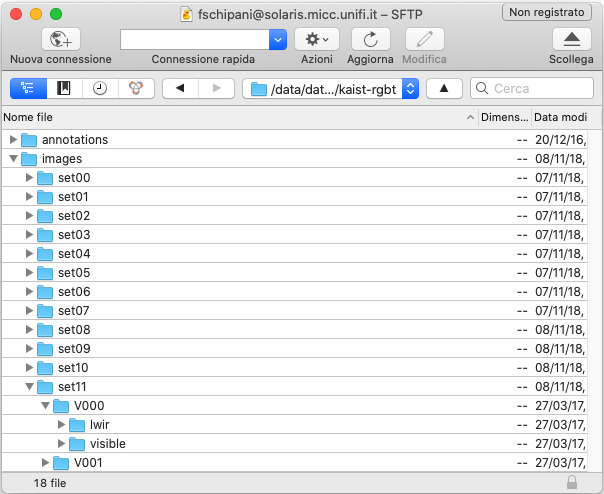
\includegraphics[width=0.7\textwidth]{images/screen_kaist.png}
    \caption{Suddivisione del dataset KAIST MPD}
    \label{fig:kaist_dataset_folder}
\end{figure} 
Il dataset in questione ha già una divisione predefinita tra train set e test set, ottenibile eseguendo uno script presente nella cartella del dataset. 

La successiva operazione che è stata effettuata è la stesura di uno script per convertire questi suddetti file in un formato accettato dalla specifica implementazione di RetinaNet utilizzata, ovvero un \texttt{CSV} composto da colonne contenenti in ordine il path dell'immagine, le coordinate dell'eventuale e la classe dell'eventuale \ac{BB}. 

In questo dataset, come detto in Sezione \ref{subsec:kmpd}, sono presenti le classi \texttt{person}, \texttt{people}, \texttt{cyclist} e \texttt{person?}. A scopo di test sono state create due varianti dei file \texttt{CSV} poco sopra descritti. La prima variante comprende solamente le \ac{BB} che contengono \texttt{person} e \texttt{cyclist}, mentre la seconda variante, usata soprattutto in fase di test comprende anche la classe \texttt{people} opportunamente rinominata alla necessità in \texttt{person}.
\paragraph{Annotazioni delle auto}
A differenza del dataset di FLIR, descritto in Sezione \ref{subsec:flirdataset}, mancano le annotazioni delle autovetture. Per effettuare altri esperimenti, descritti nelle sezioni a venire, è stato deciso di realizzarle a mano su circa $1000$ immagini. 

Al fine di rispecchiare il più possibile la divisione originale tra giorno e notte del dataset è stata necessaria un'analisi più approfondita della struttura stessa, da cui è derivato che ci sono in numero molto simile immagini diurne e notturne. Per il dettaglio della suddivisione si può far riferimento a Tabella \ref{table:day_night_kaist}.
\begin{table}[]
    \begin{tabular}{c|cccccc}
    Diurne & SET00 & SET01 & SET02 & SET06 & SET07 & SET08 \\ \hline
    Notturne & SET03 & SET04 & SET05 & SET09 & SET10 & SET11
    \end{tabular}
    \caption{Suddivisione giorno notte di KAIST}
    \label{table:day_night_kaist}
\end{table}
Dopodiché sono state selezionate casualmente $200$ immagini per ognuna delle cartelle \texttt{SET00/V000}, \texttt{SET05/V000}, \texttt{SET06/V001}, \texttt{SET08/V000} e \texttt{SET09/V000}. 

Tramite lo strumento \ac{VIA} \cite{dutta2019vgg, dutta2016via} messo a disposizione gratuitamente sono state annotate tutte le auto, furgoni e bus non eccessivamente occlusi. Infine sono state prese le immagini di \texttt{SET00/V000} e \texttt{SET05/V000} per formare un piccolo train set, mentre quelle di \texttt{SET08/V000} e \texttt{SET09/V000} sono state usate per il test set. Il validation set è stato fatto con il \texttt{SET06/V001}. 

\subsection{FLIR Thermal Starter Dataset}
\label{subsec:flir_experiment}
Il dataset di FLIR ha richiesto molto poco preprocessing in quanto è stato sufficiente scrivere uno script che convertisse le annotazioni fornite con il dataset in un formato usabile da RetinaNet. In Codice \ref{code:flir_conversion} è possibile vedere il suddetto script. L'unica accortezza usata è stata di selezionare solamente un sottoinsieme delle annotazioni, ovvero \texttt{people}, \texttt{bycicles} e \texttt{cars}. Questo è stato fatto per far coincidere il più possibile le annotazioni di questo dataset con quelle del dataset di Sezione \ref{subsec:kaist_experiment}.

\begin{lstlisting}[caption={Script di conversione per dataset FLIR}, language=Python, basicstyle=\tiny,label=code:flir_conversion]
import json
import glob
import csv
import itertools
import progressbar
if __name__ == "__main__":
    annotations_path = '/data/datasets/FLIR_ADAS/FLIR_ADAS/training/Annotations/*.json'
    id_to_name = {
        '1': 'People',
        '2': 'Bicycles',
        '3': 'Cars',
        '18': 'Dogs',
        '91': 'Other'
    }
    tot = len(glob.glob(annotations_path))
    bar = progressbar.ProgressBar(maxval=tot, widgets=[progressbar.Bar('=', '[', ']'), ' ', progressbar.Percentage()])
    i = 0
    bar.start()
    with open('thermal_validation_KAIST_TRAIN_WCARS.csv', 'w' ) as csvfile:
        filewriter = csv.writer(csvfile, delimiter=',', quotechar='|', quoting=csv.QUOTE_MINIMAL)
        for file_name in glob.iglob(annotations_path):
            data = json.load(open(file_name))
            if len(data['annotation'])>0:
                for i in range(len(data['annotation'])):
                    if data['annotation'][i]['category_id'] in ['1', '2', '3']:
                        x1, y1 = data['annotation'][i]['segmentation'][0][0],data['annotation'][i]['segmentation'][0][1]
                        x2, y2 = data['annotation'][i]['segmentation'][0][4],data['annotation'][i]['segmentation'][0][5]
                        filewriter.writerow([file_name.replace('Annotations', 'PreviewData')]+[x1, y1, x2, y2]+[id_to_name[data['annotation'][i]['category_id']]])
            else:
                filewriter.writerow([file_name, '',  '', '', '', ''])
            i = i+1
            bar.update(i)
    bar.finish()
  
\end{lstlisting}

\subsection{Video di Rete Ferroviaria Italiana}
\label{subsec:rfi_video_experiment}
I video termici forniti per il progetto di ricerca della tesi sono stati girati da telecamere \textit{Foshvision FS-UV535R104A Thermal Bi-spectrum} e \textit{HikVision DS-2TD2866-25 Thermal Bi-spectrum Network Bullet Camera} sul circuito di test di \ac{RFI} di San Donato a Bologna.
Il formato in cui sono stati forniti è \texttt{mp4}, quindi per renderli usabili da RetinaNet è stato reso necessario l'utilizzo del software \texttt{ffmpeg} per estrarre i singoli frame. 

Per realizzare una fase di fine tuning sulla rete, analogamente a quello fatto in Sezione \ref{subsec:kaist_experiment}, sono stati annotati manualmente degli operai a lavoro su un unico video.
Il video in questione, della durata di circa $15$ minuti può essere segmentato in tre parti. La prima, che arriva circa fino al minuto $8$ non contiene alcun operaio o oggetto su cui è possibile realizzare annotazioni. La seconda parte, che inizia dal minuto 8 e si conclude quasi alla fine, vede degli operai che lavorano sulla linea ferroviaria. L'ultima parte è simile alla prima in quanto gli operai hanno finito il loro lavoro e non sono più nella scena ripresa dalla telecamera. 
Sempre come in Sezione \ref{subsec:kaist_experiment} sono state selezionate casualmente delle immagini. Dalla prima parte del video sono state selezionate $200$ immagini, dalla seconda $400$ e dall'ultima che è la più corta $100$. Le annotazioni anche in questo caso sono state realizzate con \ac{VIA}, solamente sulla seconda parte di video e solamente con la classe \texttt{person}.
 

\section{Esperimenti iniziali su immagini termiche}
\label{sec:init_experiment_thermal}
Riprendendo il discorso di Sezione \ref{sec:addestramento_iniziale_di_retinanet} si parlerà ora dei vari esperimenti effettuati con i vari dataset a disposizione. 




\paragraph{Test dei pesi di KAIST su FLIR}
La prima di queste sperimentazioni è stata provare i risultati di Sezione \ref{subsec:rgb_to_thermal_kaist} sul dataset di FLIR. Il test è stato effettuato provando diverse soglie di rilevazione che variano tra $0.3$ a $0.8$ con passo di $0.1$. Il grafico di Figura \ref{fig:map_first_flir_lwir} riassume i risultati. 
\begin{figure}[]
    \centering
    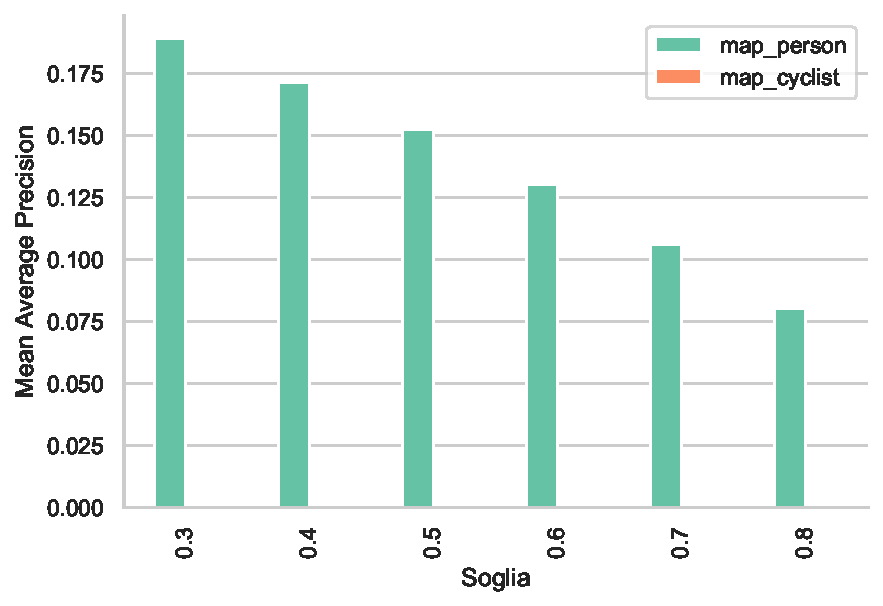
\includegraphics[width = 0.9\textwidth]{images/graphic/first_test_lwir_map.pdf}
    \caption{MAP al variare del valore di soglia su FLIR}
    \label{fig:map_first_flir_lwir}
\end{figure}
I risultati sono abbastanza deludenti, soprattutto sul fronte della rilevazione dei ciclisti. La motivazione principale è la carenza di esempi sui ciclisti in quanto ce ne sono molti pochi rispetto ad esempio i pedoni, un'altra motivazione degli scarsi risultati ottenuti è imputabile al diverso formato dell'annotazione in quanto su FLIR la \ac{BB} viene posta solamente sul ciclista, mentre su \ac{kmpd} sul ciclista più il mezzo. I risultati migliori comunque si ottengono con una soglia pari a $0.3$, in Figura \ref{fig:examples_first} mostriamo alcuni esempi di immagini annotate e classificate da Retinanet, mentre in Tabella \ref{tab:first_experiment_flir} sono presenti i valori più dettagliati rispetto al miglior risultato. 
\begin{figure}[]
    \centering
    \makebox[\textwidth]{
    \subfloat{
        \begin{minipage}[b][][t]{.3\textwidth}
        \centering
        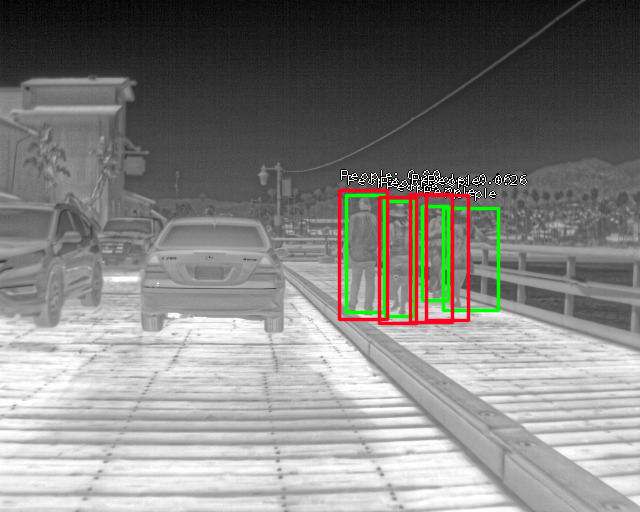
\includegraphics[width=.8\textwidth]{images/examples/first_flir_test/10.png}
        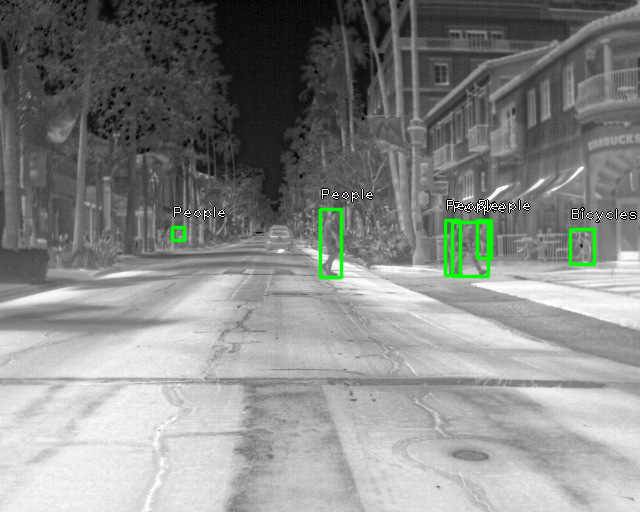
\includegraphics[width=.8\textwidth]{images/examples/first_flir_test/21.png}
        \end{minipage}
    }%
    \subfloat{
        \begin{minipage}[b][][t]{.3\textwidth}
        \centering
        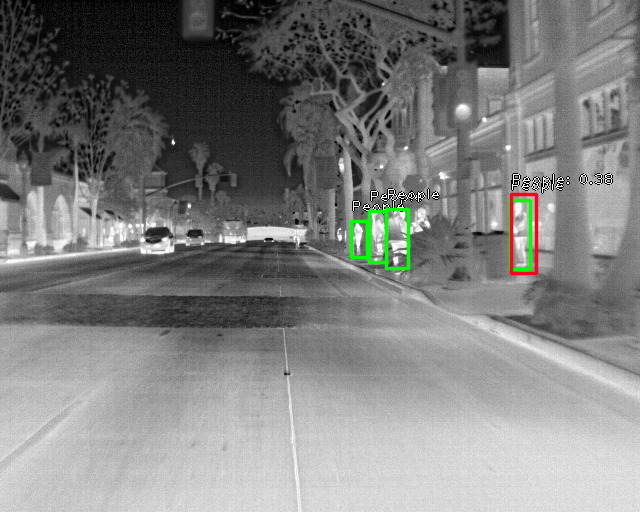
\includegraphics[width=.8\textwidth]{images/examples/first_flir_test/28.png}
        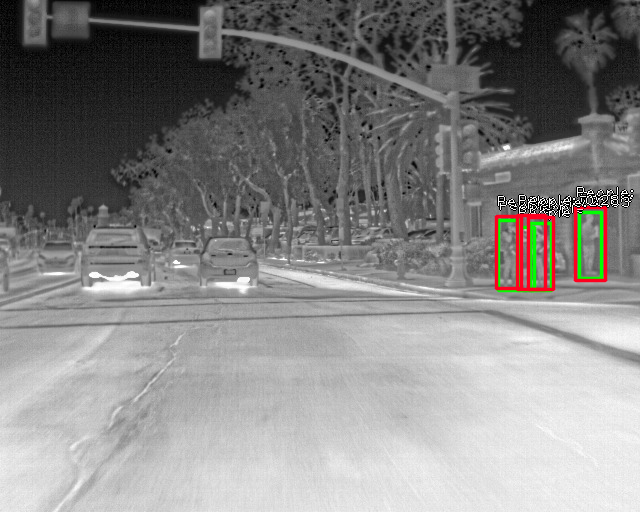
\includegraphics[width=.8\textwidth]{images/examples/first_flir_test/35.png}
        \end{minipage}
    }
    \subfloat{
        \begin{minipage}[b][][t]{.3\textwidth}
        \centering
        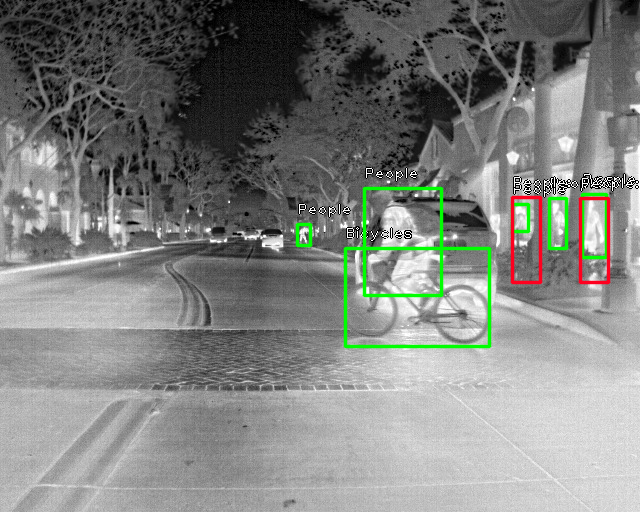
\includegraphics[width=.8\textwidth]{images/examples/first_flir_test/39.png}
        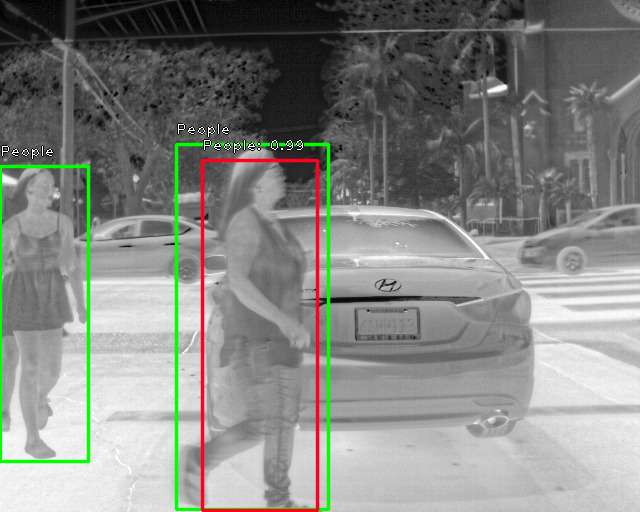
\includegraphics[width=.8\textwidth]{images/examples/first_flir_test/8.png}
        \end{minipage}
    }
    }
    \caption{Esempio di predizioni, in verde la \textit{ground truth} in rosso le predizioni.} 
    \label{fig:examples_first} 
\end{figure} 
\begin{table}[]
    \centering
    \begin{tabular}{c|c|c|}
    \cline{2-3}
     & Istanze & Map \\ \hline
    \multicolumn{1}{|c|}{Person} & 5779 & 0.1889 \\ \hline
    \multicolumn{1}{|c|}{Cyclist} & 471 & 0.0001 \\ \hline
    \multicolumn{1}{|c|}{Complessivo} & 6250 & 0.1747 \\ \hline
    \end{tabular}
    \caption{Risultati del primo esperimento su FLIR}
    \label{tab:first_experiment_flir}
\end{table}
La Figura \ref{fig:precision_recall_person_1} mostra la curva di precision-recall al variare della soglia, e si nota immediatamente una mancanza sia di precisione che di richiamo. Infatti se abbiamo maggior esempi classificati per una soglia più bassa otteniamo una scarsa precisione, situazione contraria si verifica invece quando si aumenta la soglia di rilevamento.  
\begin{figure}[]
    \centering
    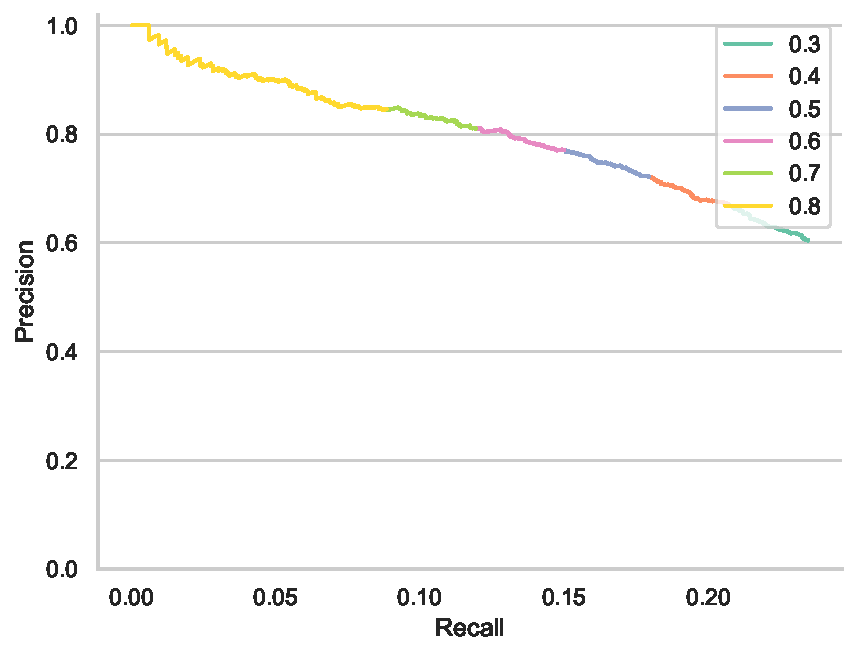
\includegraphics[width=\textwidth]{images/graphic/precision_recall_test_flir_kaist.pdf}
    \caption{Precision-Recall per classe \texttt{person}}
    \label{fig:precision_recall_person_1}
\end{figure}





\paragraph{Addestramento su FLIR partendo da COCO}
In questo esperimento si effettua una fase di addestramento di RetinaNet partendo dai pesi della rete preaddestrata su \ac{MSCOCO}. Dare questo tipo di imprinting al nostro modello permette di effettuare un'operazione considerabile alla stessa stregua del Transfer Learning, e di ridurre quindi sensibilmente i tempi di addestramento. Il grafico della fase di addestramento è in Figura \ref{fig:train_from_coco_FLIR} e come è possibile vedere le varie loss sono scese fino ad arrivare quasi a convergenza verso l'epoca $45$. La discesa è più stabile rispetto a quella vista in Sezione \ref{subsec:rgb_to_thermal_kaist} e questo è probabilmente dovuto alla migliore qualità di immagini di FLIR rispetto a \ac{kmpd}.  
\begin{figure}[]
    \centering
    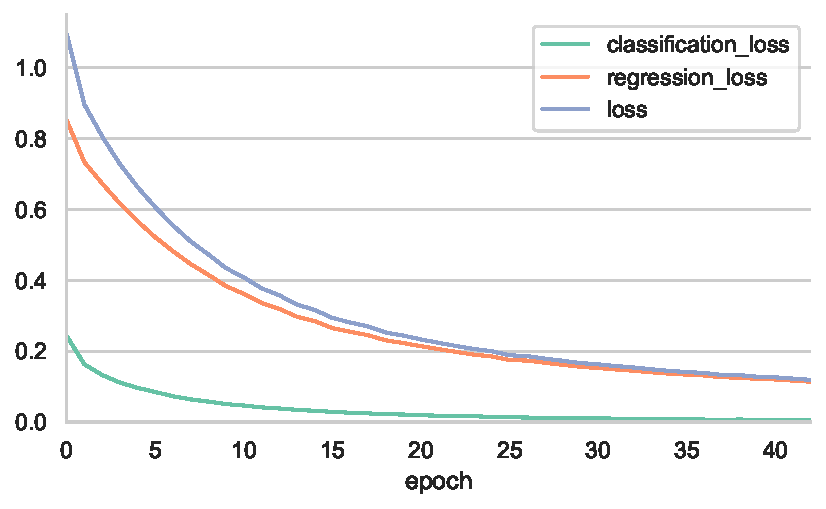
\includegraphics[width = \textwidth]{images/graphic/train_flir_from_coco.pdf}
    \caption{Addestramento di RetinaNet su FLIR partendo dai pesi di COCO}
    \label{fig:train_from_coco_FLIR}
\end{figure}
La fase di test dei pesi risultati di questo modello sono stati testati sul dataset di FLIR ottenendo i risultati in Figura \ref{fig:map_flir_from_coco}. 
\begin{figure}[]
    \centering
    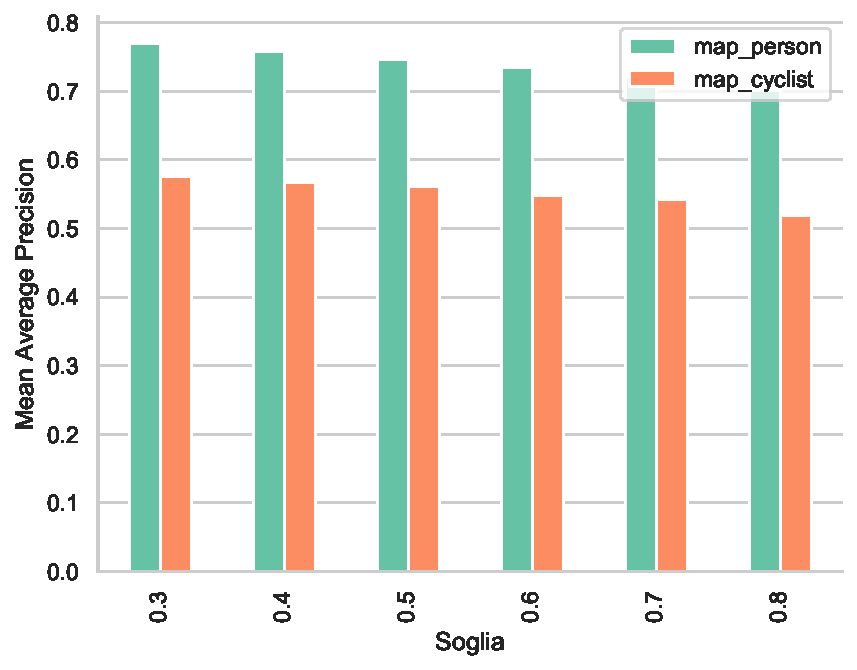
\includegraphics[width=\textwidth]{images/graphic/flir_from_coco_map.pdf}
    \caption{\ac{map} su FLIR addestrato dai pesi di COCO}
    \label{fig:map_flir_from_coco}
\end{figure}
Rispetto ai risultati mostrati in precedenza si ha un incremento notevole della \ac{map}. Come prima si verifica anche lo stesso fenomeno per cui si ottiene maggior \ac{map} con una soglia più bassa, ma a discapito della qualità delle rilevazioni. Si può osservare questo fenomeno guardando la curva di precision-recall in Figura \ref{fig:precision_recall_curve_flir_coco}. In Tabella \ref{table:coco_result_best_flir} sono presenti i risultati migliori ottenuti in termini di \ac{map}. 
\begin{figure}[]
    \centering
    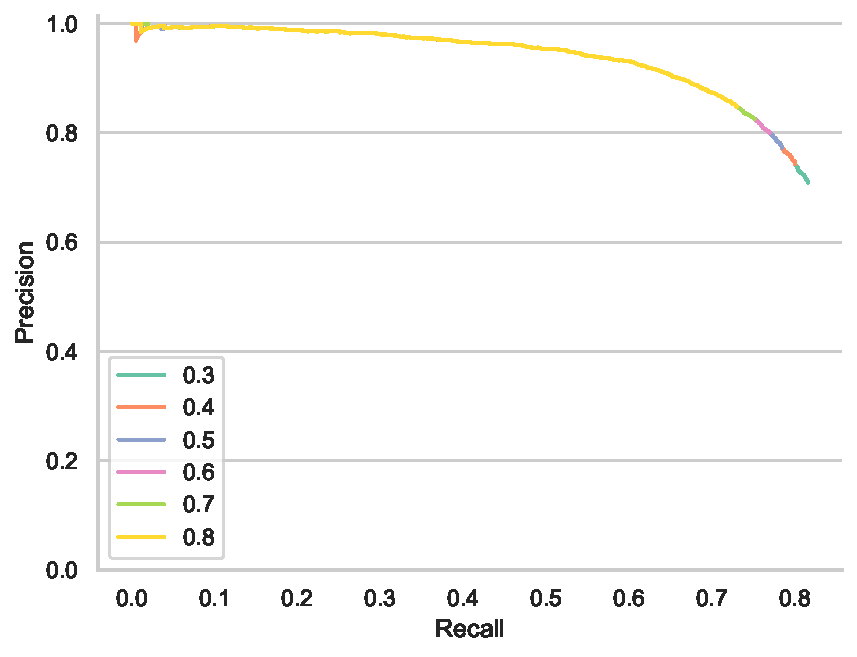
\includegraphics[width = \textwidth]{images/graphic/flir_coco_pr.pdf}
    \caption{Curva P/R di FLIR addestrato partendo da COCO (\texttt{person})}
    \label{fig:precision_recall_curve_flir_coco}
\end{figure}

\begin{table}[]
    \centering
    \begin{tabular}{c|c|c|}
    \cline{2-3}
     & Istanze & Map \\ \hline
    \multicolumn{1}{|c|}{Person} & 5779 & 0.575442 \\ \hline
    \multicolumn{1}{|c|}{Cyclist} & 471 & 0.769743 \\ \hline
    \multicolumn{1}{|c|}{Complessivo} & 6250 & 0.672592 \\ \hline
    \end{tabular}
    \caption{Risultati di FLIR da COCO con soglia $0.3$}
    \label{table:coco_result_best_flir}
\end{table}


\paragraph{Addestramento di FLIR partendo da KAIST}
L'idea dietro questo esperimento fonda le sue basi dietro al fallimento riguardante un test precedente, ovvero quello in cui si testano i pesi di \ac{kmpd} sul dataset di FLIR. L'evoluzione delle misure di loss durante l'addestramento è visibile in Figura \ref{fig:flir_train_from_kaist}. La prima cosa che si nota è l'andamento molto simile rispetto all'esperimento precedente, successivamente si può notare anche come si arriva ai medesimi risultati, ma con qualche epoca di anticipo. Infatti, nonostante i valori di partenza delle loss sono sensibilmente più elevati si ha una discesa più repentina. Grafici analoghi ai precedenti è possibile vederli in Figura \ref{fig:flir_train_from_kaist_pr} e \ref{fig:flir_train_from_kaist_result}. L'andamento è comunque analogo al precedente, ma come si può vedere da Tabella \ref{table:best_flir_from_kaist} si ottiene un calo delle performance sotto il punto di vista della \ac{map}. 
\begin{figure}[]
    \centering
    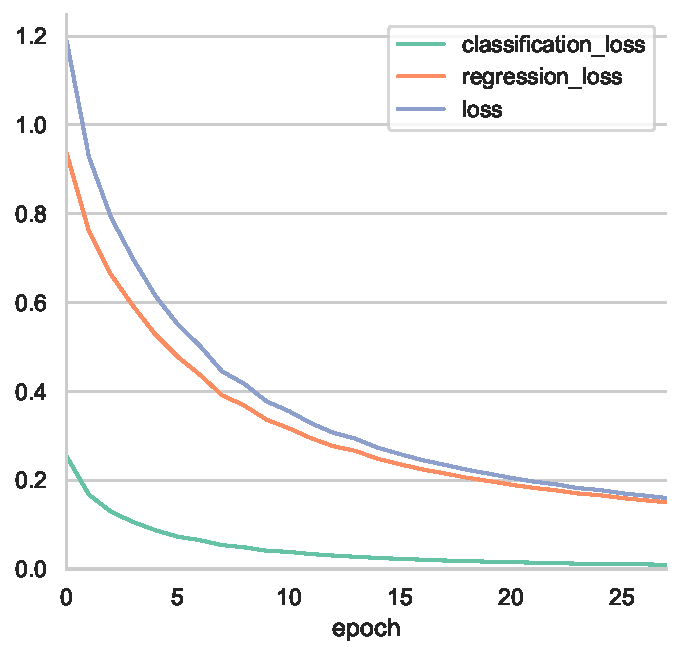
\includegraphics[width=0.9\textwidth]{images/graphic/flir_from_kaist.pdf}
    \caption{Addestramento su FLIR partendo dai pesi di KAIST}
    \label{fig:flir_train_from_kaist}
\end{figure}
\begin{figure}[]
    \centering
    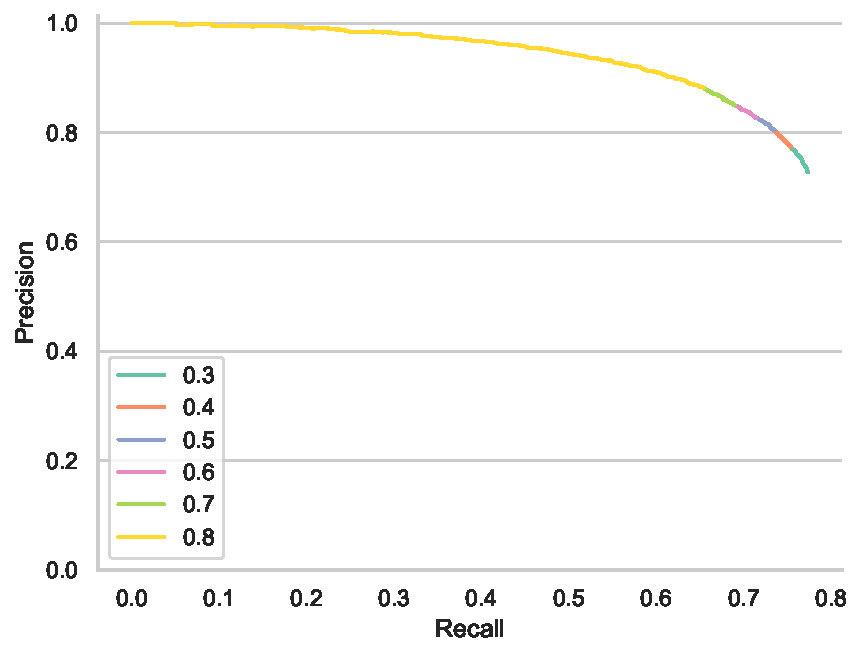
\includegraphics[width=0.9\textwidth]{images/graphic/flir_from_kaist_pr.pdf}
    \caption{Grafico P/R dell'addestramento su FLIR partendo dai pesi di KAIST (\texttt{person})}
    \label{fig:flir_train_from_kaist_pr}
\end{figure}
\begin{figure}[]
    \centering
    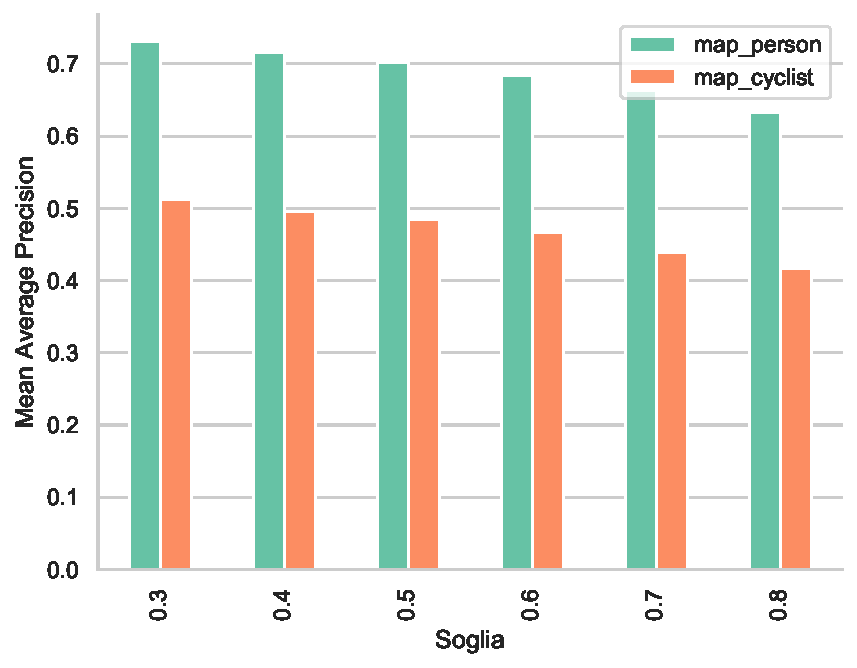
\includegraphics[width=0.9\textwidth]{images/graphic/flir_from_kaist_result.pdf}
    \caption{Risultati dell'addestramento su FLIR partendo dai pesi di KAIST}
    \label{fig:flir_train_from_kaist_result}
\end{figure}
\begin{table}[]
    \centering
    \begin{tabular}{c|c|c|}
    \cline{2-3}
     & Istanze & Map \\ \hline
    \multicolumn{1}{|c|}{Person} & 5779 & 0.512462 \\ \hline
    \multicolumn{1}{|c|}{Cyclist} & 471 & 0.730898 \\ \hline
    \multicolumn{1}{|c|}{Complessivo} & 6250 & 0.621680 \\ \hline
    \end{tabular}
    \caption{Risultati migliori dell'addestramento su FLIR partendo dai pesi di KAIST, soglia $0.3$}
    \label{table:best_flir_from_kaist}
\end{table}


\paragraph{Test dei pesi migliori su KAIST} %FLIR_FROM_COCO_43.h5, imageSets/csv_files_NO_PEOPLE/lwir/test-night-01-no-people.csv, class_name_to_id_NO_PEOPLE.csv DESCRIVERE FIGURE
Per ora i pesi migliori ottenuti in termini di \ac{map} sulle persone è stato ottenuto addestrando RetinaNet sul dataset di FLIR partendo dai pesi della rete preaddestrata su \ac{MSCOCO}. Proviamo ora a vedere cosa succede testando questi pesi sul dataset di \ac{kmpd} in un caso che è già stato visto essere favorevole alla detection tramite immagini termiche, ovvero quando le acquisizioni sono state effettuate di notte.



\begin{figure}
    \begin{minipage}{.5\linewidth}
        \centering
        \subfloat[P/R su \texttt{person}]{
            \label{main:a}
            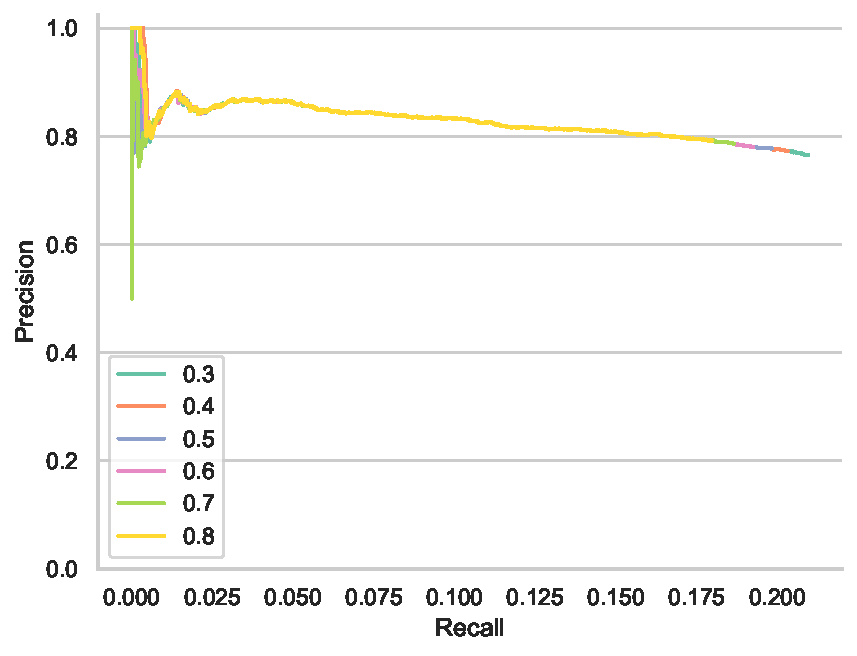
\includegraphics[scale=.5]{images/graphic/FLIR_FROM_COCO_PERSON.pdf}
        }
    \end{minipage}%
    \begin{minipage}{.5\linewidth}
        \centering
        \subfloat[\ac{map} su \texttt{person}]{
            \label{main:b}
            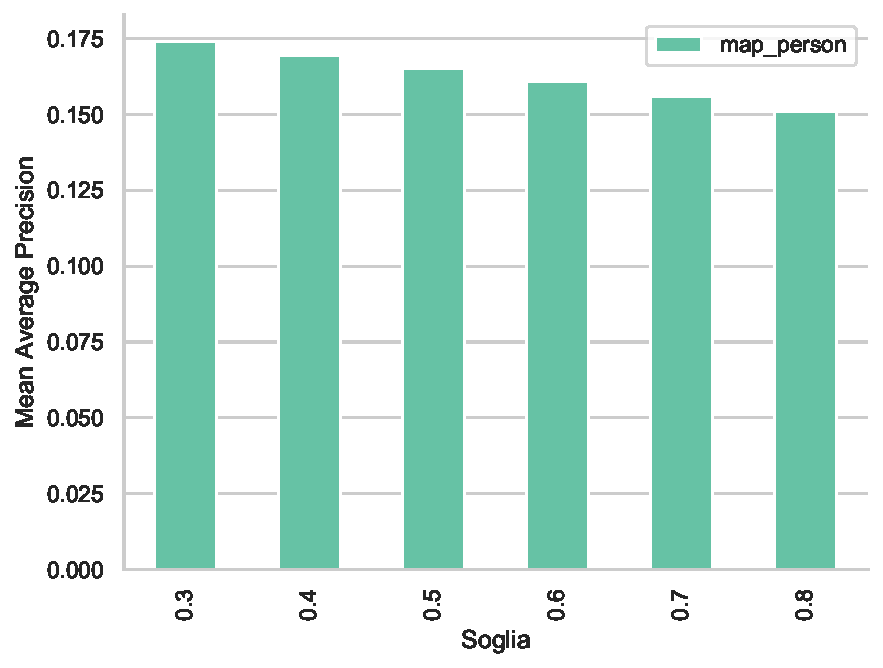
\includegraphics[scale=.5]{images/graphic/FLIR_FROM_COCO_RESULTS.pdf}
            }
    \end{minipage}
    \centering
    \caption{Test su KAIST del risultato migliore su FLIR}
    \label{fig:main}
\end{figure}

In Figura \ref{fig:main} è possibile visionare un sunto dei risultati ottenuti. Si può osservare in particolare nella parte \ref{main:b} che la \ac{map} ottenuta è molto bassa. Questa scarsa precisione in fase di inferenza porta a non avere grandi risultati all'atto pratico, basti vedere anche la Figura \ref{main:a} per notare come la curva di Precision/Recall indichi una forte penuria nella Recall. 
Dati alla mano si può dire sicuramente che le rilevazioni effettuate sono corrette, ma in pratica ne vengono trovate molte poche rispetto al totale. 

\paragraph{Rilevazione delle auto} %riferimento in TODO -> "Per 5/10" DESCRIVERE ULTIME FIGURE
La rilevazione delle auto su entrambi i dataset ha richiesto un lavoro di preprocessing sul dataset \ac{kmpd} descritto in precedenza nella Sezione \ref{subsec:kaist_experiment}.
Il primo test effettuato è fissare una baseline data dall'addestramento su FLIR ed il successivo test sulla parte di dataset annotata manualmente di \ac{kmpd} cercando di vedere il comportamento con le autovetture. Il risultato è in Tabella \ref{table:baseline_car_kaist}. 
\begin{table}[]
    \centering
    \begin{tabular}{c|c|c|}
    \cline{2-3}
     & Istanze & Map \\ \hline
    \multicolumn{1}{|c|}{Person} & 755 & 0.3730 \\ \hline
    \multicolumn{1}{|c|}{Cyclist} & 15 & 0 \\ \hline
    \multicolumn{1}{|c|}{Cars} & 1088 & 0.5716 \\ \hline
    \multicolumn{1}{|c|}{Complessivo} & 6250 & 0.4863 \\ \hline
    \end{tabular}
    \caption{Baseline per la rilevazione di vetture su KAIST}
    \label{table:baseline_car_kaist}
\end{table} 

Il passo successivo è stata una fase di \textit{fine tuning} di questi pesi sulla parte di train di \ac{kmpd} annotata manualmente con le vetture. Come si può vedere in Figura \ref{fig:fine_tuning_kaist_flir} l'addestramento ha avuto una durata relativamente corta in quanto con solamente $15$ ore e $18$ epoche è arrivato al termine.
\begin{figure}[]
    \centering
    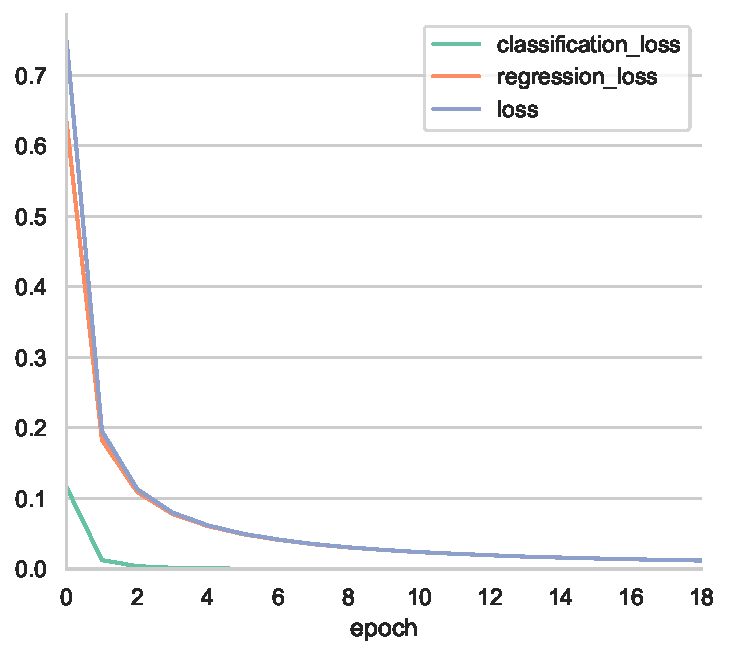
\includegraphics[width=\textwidth]{images/graphic/fine_tuning_kaist_flir.pdf}
    \caption{Fine tuning di KAIST partendo da FLIR}
    \label{fig:fine_tuning_kaist_flir}
\end{figure}
Vista la repentina discesa delle loss e la scarsità di dati a disposizione è facile incorrere in un fenomeno di overfitting, ed infatti è quello che è accaduto. In Tabella \ref{tab:fine_tuning_kaist_flir} sono mostrati i risultati per alcune epoche di questa fase di addestramento, in grassetto ci sono i risultati migliori per ogni categoria. Come si può vedere nell'epoca $18$, ovvero l'ultima, non si raggiungono picchi di \ac{map}, il che è un sintomo di scarsa capacità di generalizzazione. Riguardo la classe \texttt{person} e \texttt{cyclist} il risultato migliore si ha all'epoca $8$. Invece riguardo la rilevazione di automobili si ha il risultato migliore all'epoca $10$. Si può notare inoltre che sia riguardo le persone che le automobili c'è stato un incremento nelle prestazioni della detection (Tabella \ref{tab:fine_tuning_kaist_flir_increment}). 
\begin{table}[]
    \centering
    \begin{tabular}{c|c|c|c|c|c|}
    \cline{2-6}
     & EP 18 & EP 10 & EP 09 & EP 08 & EP 05 \\ \hline
    \multicolumn{1}{|c|}{Person (755)} & 0.4964 & 0.5050 & 0.5018 & \textbf{0.5137} & 0.5048 \\ \hline
    \multicolumn{1}{|c|}{Cyclist (15)} & 0.0333 & 0.0444 & 0.0667 & \textbf{0.1000} & 0.0667 \\ \hline
    \multicolumn{1}{|c|}{Cars (1088)} & 0.6767 & \textbf{0.6929} & 0.6854 & 0.6787 & 0.6870 \\ \hline
    \multicolumn{1}{|c|}{Complessivo} & 0.5983 & \textbf{0.6113} & 0.6058 & 0.6070 & 0.6080 \\ \hline
    \end{tabular}
    \caption{Risultati del fine tuning su kaist annotato manualmente}
    \label{tab:fine_tuning_kaist_flir}
\end{table}
\begin{table}[]
    \centering
    \begin{tabular}{c|c|c|c|}
    \cline{2-4}
     & Post & Pre & Incremento \\ \hline
    \multicolumn{1}{|c|}{Person (755)} & 0.5137 & 0.3730 & +37\% \\ \hline
    \multicolumn{1}{|c|}{Cyclist (15)} & 0.1000 & 0.000 & + \\ \hline
    \multicolumn{1}{|c|}{Cars (1088)} & 0.6929 & 0.5716 & +21\% \\ \hline
    \multicolumn{1}{|c|}{Complessivo} & 0.6113 & 0.4863 & +25\% \\ \hline
    \end{tabular}
    \caption{Incremento rispetto alla baseline dopo fine tuning}
    \label{tab:fine_tuning_kaist_flir_increment}
\end{table}

In particolare possiamo andare ad analizzare le performance ottenute all'epoca 8 in quanto risultano mediamente le migliori. In Figura \ref{fig:test_kaist_ep8} sono presenti le curve di Precision/Recall sulla classe \texttt{person} e \texttt{cars}, mentre in Figura \ref{fig:test_kaist_ep8_map} sono presenti i grafici di \ac{map} al variare della soglia di rilevamento. Non è stata analizzata in maniera più dettagliata la classe \texttt{cyclist} in quanto gli esempi sono troppi pochi per ottenere risultati significativi. 

Andando a confrontare le curve di P/R di Figura \ref{fig:test_kaist_ep8} si nota come sulle automobili si hanno in media rilevazioni più precise ed anche un richiamo maggiore, il che porta ad avere detection sulle vetture in generale migliori rispetto a quelle ottenute sui pedoni. Il motivo presumibilmente può essere imputato ad una maggior somiglianza tra l'aspetto delle vetture in immagini termiche rispetto a quello che possono avere dei pedoni.  
\begin{figure}
    \begin{minipage}{.5\linewidth}
        \centering
        \subfloat[P/R su \texttt{person}]{
            \label{test_kaist_ep8:a}
            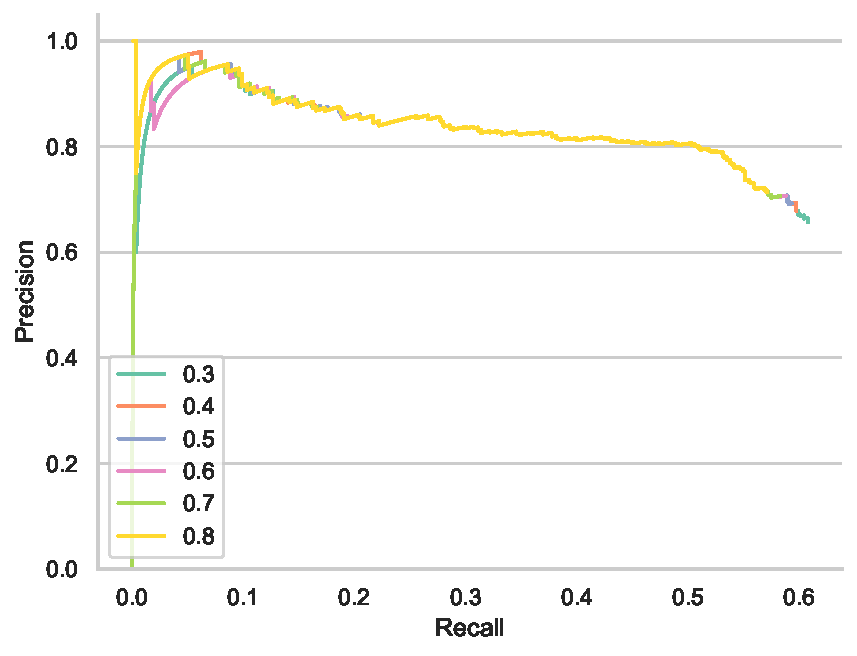
\includegraphics[scale=.5]{images/graphic/graphics_manual_annotations_08_person.pdf}
        }
    \end{minipage}%
    \begin{minipage}{.5\linewidth}
        \centering
        \subfloat[P/R su \texttt{cars}]{
            \label{test_kaist_ep8:b}
            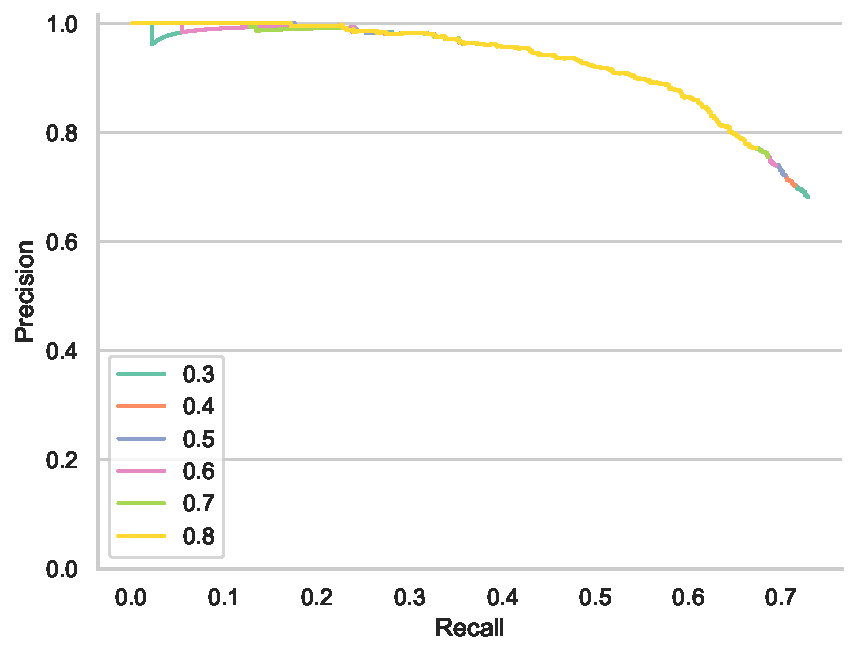
\includegraphics[scale=.5]{images/graphic/graphics_manual_annotations_08_cars.pdf}
            }
    \end{minipage}
    \centering
    \caption{P/R su KAIST all'epoca 8}
    \label{fig:test_kaist_ep8}
\end{figure}



\begin{figure}[]
    \centering
    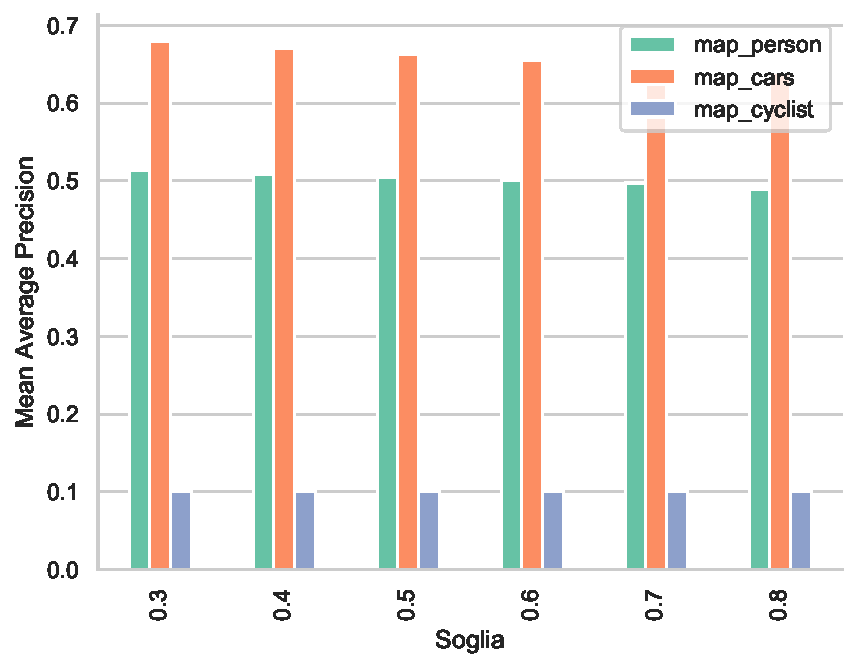
\includegraphics[width=\textwidth]{images/graphic/graphics_map.pdf}
    \caption{Fine tuning di KAIST partendo da FLIR}
    \label{fig:test_kaist_ep8_map}
\end{figure}

\section{Data Augmentation}
\label{sec:data_augmentaion_experiment}
Al fine di migliorare la detection degli esseri umani un ulteriore diramazione di esperimenti è stata svolta usando tecniche di Data Augmentation (Sezione \ref{sec:data_augmentation}). Le tecniche utilizzate in particolare sono AutoAugment, RandAugment ed infine delle immagini termiche generate da una \ac{GAN}. 
\paragraph{AutoAugment}
AutoAugment per via dell'elevata richiesta computazionale, non alla portata dell'hardware utilizzato per lo sviluppo della tesi, non è stato sfruttato adeguatamente, bensì sono state usate policy derivanti dagli addestramenti effettuati su altri dataset. In Codice \ref{code:policy_v0}, \ref{code:policy_v1} e \ref{code:policy_v2} sono presenti le tre politiche di AutoAugment con cui sono stati effettuati gli esperimenti.  

\begin{lstlisting}[caption={Policy V0 di AutoAugment}, language=Python, basicstyle=\tiny,label=code:policy_v0]
def policy_v0():
  policy = [
      [('TranslateX_BBox', 0.6, 4), ('Equalize', 0.8, 10)],
      [('TranslateY_Only_BBoxes', 0.2, 2), ('Cutout', 0.8, 8)],
      [('Sharpness', 0.0, 8), ('ShearX_BBox', 0.4, 0)],
      [('ShearY_BBox', 1.0, 2), ('TranslateY_Only_BBoxes', 0.6, 6)],
      [('Rotate_BBox', 0.6, 10), ('Color', 1.0, 6)],
  ]
  return policy
\end{lstlisting}
La prima policy è la più semplice tra le tre, contiene al suo interno solamente cinque subpolicy formate a loro volta da due operazioni.
\begin{lstlisting}[caption={Policy V1 di AutoAugment}, language=Python, basicstyle=\tiny,label=code:policy_v1]
def policy_v1():
    policy = [
        [('TranslateX_BBox', 0.6, 4), ('Equalize', 0.8, 10)],
        [('TranslateY_Only_BBoxes', 0.2, 2), ('Cutout', 0.8, 8)],
        [('Sharpness', 0.0, 8), ('ShearX_BBox', 0.4, 0)],
        [('ShearY_BBox', 1.0, 2), ('TranslateY_Only_BBoxes', 0.6, 6)],
        [('Rotate_BBox', 0.6, 10), ('Color', 1.0, 6)],
        [('Color', 0.0, 0), ('ShearX_Only_BBoxes', 0.8, 4)],
        [('ShearY_Only_BBoxes', 0.8, 2), ('Flip_Only_BBoxes', 0.0, 10)],
        [('Equalize', 0.6, 10), ('TranslateX_BBox', 0.2, 2)],
        [('Color', 1.0, 10), ('TranslateY_Only_BBoxes', 0.4, 6)],
        [('Rotate_BBox', 0.8, 10), ('Contrast', 0.0, 10)],
        [('Cutout', 0.2, 2), ('Brightness', 0.8, 10)],
        [('Color', 1.0, 6), ('Equalize', 1.0, 2)],
        [('Cutout_Only_BBoxes', 0.4, 6), ('TranslateY_Only_BBoxes', 0.8, 2)],
        [('Color', 0.2, 8), ('Rotate_BBox', 0.8, 10)],
        [('Sharpness', 0.4, 4), ('TranslateY_Only_BBoxes', 0.0, 4)],
        [('Sharpness', 1.0, 4), ('SolarizeAdd', 0.4, 4)],
        [('Rotate_BBox', 1.0, 8), ('Sharpness', 0.2, 8)],
        [('ShearY_BBox', 0.6, 10), ('Equalize_Only_BBoxes', 0.6, 8)],
        [('ShearX_BBox', 0.2, 6), ('TranslateY_Only_BBoxes', 0.2, 10)],
        [('SolarizeAdd', 0.6, 8), ('Brightness', 0.8, 10)],
    ]
    return policy
\end{lstlisting}
La seconda, a differenza della prima introduce un numero di subpolicy più alto, ma mantiene il numero di operazioni applicabili ad immagine. 

\begin{lstlisting}[caption={Policy V2 di AutoAugment}, language=Python, basicstyle=\tiny,label=code:policy_v2]
def policy_v2():
    policy = [
        [('Color', 0.0, 6), ('Cutout', 0.6, 8), ('Sharpness', 0.4, 8)],
        [('Rotate_BBox', 0.4, 8), ('Sharpness', 0.4, 2),
         ('Rotate_BBox', 0.8, 10)],
        [('TranslateY_BBox', 1.0, 8), ('AutoContrast', 0.8, 2)],
        [('AutoContrast', 0.4, 6), ('ShearX_BBox', 0.8, 8),
         ('Brightness', 0.0, 10)],
        [('SolarizeAdd', 0.2, 6), ('Contrast', 0.0, 10),
         ('AutoContrast', 0.6, 0)],
        [('Cutout', 0.2, 0), ('Solarize', 0.8, 8), ('Color', 1.0, 4)],
        [('TranslateY_BBox', 0.0, 4), ('Equalize', 0.6, 8),
         ('Solarize', 0.0, 10)],
        [('TranslateY_BBox', 0.2, 2), ('ShearY_BBox', 0.8, 8),
         ('Rotate_BBox', 0.8, 8)],
        [('Cutout', 0.8, 8), ('Brightness', 0.8, 8), ('Cutout', 0.2, 2)],
        [('Color', 0.8, 4), ('TranslateY_BBox', 1.0, 6), ('Rotate_BBox', 0.6, 6)],
        [('Rotate_BBox', 0.6, 10), ('BBox_Cutout', 1.0, 4), ('Cutout', 0.2, 8)],
        [('Rotate_BBox', 0.0, 0), ('Equalize', 0.6, 6), ('ShearY_BBox', 0.6, 8)],
        [('Brightness', 0.8, 8), ('AutoContrast', 0.4, 2),
         ('Brightness', 0.2, 2)],
        [('TranslateY_BBox', 0.4, 8), ('Solarize', 0.4, 6),
         ('SolarizeAdd', 0.2, 10)],
        [('Contrast', 1.0, 10), ('SolarizeAdd', 0.2, 8), ('Equalize', 0.2, 4)],
    ]
    return policy
  
\end{lstlisting}
La terza invece diminuisce leggermente il numero di subpolicy rispetto alla seconda, ma aumenta le operazioni applicabili ad immagine a 3. 

Le seguenti politiche sono state usate per addestrare RetinaNet sulla parte di dataset di \ac{kmpd} con i label sulle vetture. Il motivo è legato al fatto che essendo le annotazioni poco numerose si prova ad aumentarne virtualmente il loro numero variandone l'aspetto tramite trasformazioni sull'immagine stessa.

Effettuando tre diverse fasi di addestramento ognuna con una policy diversa si ottengono in fase di inferenza i risultati riassunti in Tabella \ref{table:aa_kaist}. Rispetto ai risultati ottenuti in precedenza si ha un miglioramento nella rilevazione delle automobili usando la policy V0 all'epoca 5, mentre per i pedoni si ha un miglioramento nella rilevazione usando la politica V2 sempre all'epoca 5. Le variazioni tra i risultati migliori ottenuti in precedenza e quelli migliori ottenuti con AutoAugment sono riassunti in Tabella \ref{table:AA_increment}.

\begin{table}[]
    \centering
    \resizebox{\textwidth}{!}{%
    \begin{tabular}{|c|c|c|c|c|c|c|c|c|c|c|c|c|c|c|c|}
        \hline
        Policy & V0 & V0 & V0 & V1 & V1 & V1 & V1 & V1 & V1 & V2 & V2 & V2 & V2 & V2 & V2 \\ \hline
        Epoca & 5 & 8 & 11 & 5 & 10 & 15 & 20 & 30 & 33 & 05 & 10 & 15 & 20 & 30 & 37 \\ \hline
        Person (755) & 0.4808 & 0.4850 & 0.4982 & 0.5157 & 0.5005 & 0.4896 & 0.4876 & 0.4975 & 0.3873 & \cellcolor[HTML]{9AFF99}\textbf{0.5241} & 0.5032 & 0.5007 & 0.4959 & 0.5064 & 0.5064 \\ \hline
        Cyclist (15) & 0.0067 & \cellcolor[HTML]{9AFF99}\textbf{0.0167} & 0.0000 & 0.0000 & 0.0000 & 0.0000 & 0.0000 & 0.0000 & 0.0000 & 0.0000 & 0.0000 & 0.0000 & 0.0000 & 0.0000 & 0.0000 \\ \hline
        Cars (1088) & \cellcolor[HTML]{9AFF99}\textbf{0.7195} & 0.6942 & 0.6792 & 0.6805 & 0.6728 & 0.6605 & 0.6703 & 0.6693 & 0.5603 & 0.6506 & 0.6564 & 0.6505 & 0.6254 & 0.6264 & 0.6265 \\ \hline
        Complessivo & \cellcolor[HTML]{9AFF99}\textbf{0.6167} & 0.6037 & 0.6002 & 0.6080 & 0.5973 & 0.5857 & 0.5906 & 0.5941 & 0.4855 & 0.5940 & 0.5888 & 0.5844 & 0.5677 & 0.5726 & 0.5726 \\ \hline
        \end{tabular}}
    \caption{Risultati complessivi di AutoAugment su KAIST}
    \label{table:aa_kaist}
\end{table}


\begin{table}[]
    \centering
    \begin{tabular}{c|c|c|c|}
    \cline{2-4}
     & Prima di AA & Dopo AA & Variazione \\ \hline
    \multicolumn{1}{|c|}{Person (755)} & 0.5137 & 0.5241 & +2\% \\ \hline
    \multicolumn{1}{|c|}{Cyclist (15)} & 0.1000 & 0.0167 & -0.4\%\\ \hline
    \multicolumn{1}{|c|}{Cars (1088)} & 0.6929 & 0.7195 & +3.8\% \\ \hline
    \multicolumn{1}{|c|}{Complessivo} & 0.6113 & 0.6167 & +0.8\% \\ \hline
    \end{tabular}
    \caption{Incremento rispetto alla baseline dopo fine tuning}
    \label{table:AA_increment}
\end{table}

Un ulteriore esperimento effettuato con AutoAugment è relativo al miglioramento della rilevazione dei pedoni. In pratica è stata usata la politica che ha fatto ottenere un miglioramento nella rilevazione dei pedoni per effettuare un training sul dataset di FLIR. Lo scopo era di ottenere miglior capacità di generalizzazione e quindi passare da un dataset all'altro con risultati migliori. In Tabella \ref{table:tl_flir_kaist_aav2} sono presenti i risultati dell'esperimento appena descritto, mentre in Figura \ref{fig:AA_v2} è presente il grafico riguardante la progressione delle Loss durante la fase di addestramento. 
\begin{figure}[]
    \centering
    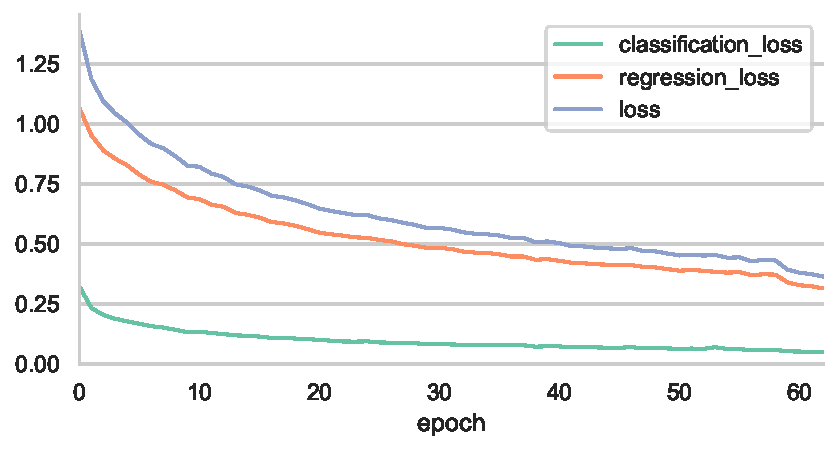
\includegraphics[width=\textwidth]{images/graphic/train_aa_flir_v2.pdf}
    \caption{Training su FLIR con policy di AutoAugment V2}
    \label{fig:AA_v2}
\end{figure}

\begin{table}[]
    \begin{tabular}{c|c|c|c|c|c|}
    \cline{2-6}
     & EP 05 & EP 20 & EP 20 & EP 50 & EP 63 \\ \hline
    \multicolumn{1}{|c|}{Person (755)} & 0.3342 & 0.2516 & 0.3619 & 0.3270 & 0.3531 \\ \hline
    \end{tabular}
    \caption{Test di transfer learning da FLIR addestrato con AA V2 a KAIST (soglia 0.3)}
    \label{table:tl_flir_kaist_aav2}
\end{table}

L'ultimo esperimento effettuato con AutoAugment parte dai pesi di quello precedentemente descritto (Figura \ref{fig:AA_v2}, Tabella \ref{table:tl_flir_kaist_aav2}) realizzando una fase di \textit{fine tuning} sul dataset di KAIST. In Tabella \ref{table:fine_tuning_aav2_kaist} sono presenti i risultati di questa ultima fase, e come si può vedere non si ottiene alcun miglioramento. 

\begin{table}[]
    \resizebox{\textwidth}{!}{%
    \begin{tabular}{c|c|c|c|c|c|c|c|c|c|}
    \cline{2-10}
     & EP 05 & EP 10 & EP 15 & EP 20 & EP 25 & EP 30 & EP 35 & EP 40 & EP 44 \\ \hline
    \multicolumn{1}{|c|}{Person (755)} & 0.5061 & 0.4899 & 0.4913 & 0.4959 & 0.4822 & 0.4847 & 0.5035 & 0.4859 & 0.4911 \\ \hline
    \multicolumn{1}{|c|}{Cyclist (15)} & 0.0000 & 0.0000 & 0.0000 & 0.0000 & 0.0000 & 0.0000 & 0.0000 & 0.0000 & 0.0000 \\ \hline
    \multicolumn{1}{|c|}{Cars (1088)} & 0.5250 & 0.5395 & 0.5360 & 0.5383 & 0.5462 & 0.5427 & 0.5454 & 0.5387 & 0.5399 \\ \hline
    \multicolumn{1}{|c|}{Complessivo} & 0.5131 & 0.5150 & 0.5135 & 0.5167 & 0.5158 & 0.5148 & 0.5239 & 0.5129 & 0.5157 \\ \hline
    \end{tabular}}
    \caption{Test dopo ulteriore fine tuning su KAIST}
    \label{table:fine_tuning_aav2_kaist}
\end{table}

\paragraph{RandAugment} 
RandAugment, come precedentemente descritto in Sezione \ref{subsec:rand_augment}, riduce notevolmente il costo computazionale rispetto ad AutoAugment per far si che si adatti al dataset su cui sarà applicato. 

In questo caso ci si hanno solo due parametri $N$ ed $M$ con il primo che indica il numero di operazioni da applicare, ed il secondo la potenza con cui applicarle. Ci si riconduce in breve ad un problema di ottimizzazione di iperparametri risolvibile anche con un algoritmo GridSearch. In questa tesi però è stata usata la piattaforma \href{http://www.comet.ml}{Comet.ml} che implementa una serie di algoritmi per realizzare ottimizzazione. L'algoritmo scelto è stato quello che loro definiscono il migliore, un algoritmo di tipo \textit{bayesiano} su cui non vengono rilasciati ulteriori dettagli.

Il target dell'ottimizzatore è la minimizzazione della \ac{map} moltiplicata per $-1$, in pratica quindi è la massimizzazione della metrica. L'intero processo ha avuto una durata di circa $130$ ore consecutive in quanto l'ambiente è stato impostato per eseguire una fase di training di $7$ epoche seguita da un test per la valutazione delle performance, partendo dai pesi di RetinaNet preaddestrata su \ac{MSCOCO}. Il tutto è stato realizzato sulla parte di dataset di \ac{kmpd} con le annotazioni delle automobili. Un sommario dell'ottimizzazione è in Figura \ref{fig:map_comet_ml} e come si può vedere i risultati migliori si ottengono ponendo $M$ con valori compresi tra $26$ e $30$ e con $N$ uguale a $3$.
\begin{figure}[]
    \centering
    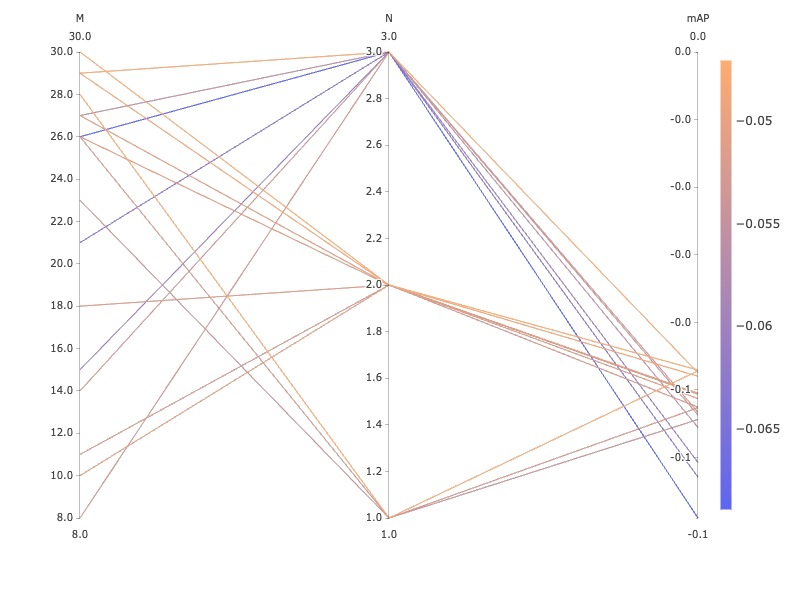
\includegraphics[width=0.9\textwidth]{images/graphic/mAP_comet.jpeg}
    \caption{\ac{map} al variare degli iperparametri}
    \label{fig:map_comet_ml}
\end{figure}

Purtroppo però non ha portato a miglioramenti probabilmente perché sette epoche non sono sufficienti partendo da pesi generici come quelli di \ac{MSCOCO}. Si ottiene una \ac{map} sulle persone pari a $0.4769$, mentre per le vetture si arriva a $0.6646$. 

\paragraph{GAN}

\section{Esperimenti su video di RFI}
\label{sec:RFI_video_experiment}

I video termici di \ac{RFI} forniti sono tre, e su tutti e tre il task è la rilevazione di persone. Inizialmente non essendo annotati l'unica operazione possibile è stata dare in pasto a RetinaNet i frame del video per realizzare inferenza usando i pesi migliori per la rilevazione di persone, ovvero quelli ottenuti tramite l'addestramento su \ac{kmpd} tramite la terza policy all'epoca 5 (Tabella \ref{table:aa_kaist}). 

I risultati iniziali, pur non potendo calcore metriche appaiono da una valutazione puramente soggettiva promettenti, in quanto le rilevazioni sembrano abbastanza precise. 

I primi test sono stati effettuati tenendo una soglia di rilevazione pari a $0.30$, questo ha portato ad una rilevazione sempre accurata degli operai, ma anche a molte rilevazioni false, come ad esempio quelle mostrate in Figura \ref{fig:rfi_030}. 

\begin{figure}[]
    \begin{minipage}{.5\linewidth}
        \centering
        \subfloat[]{
            \label{rfi_030:a}
            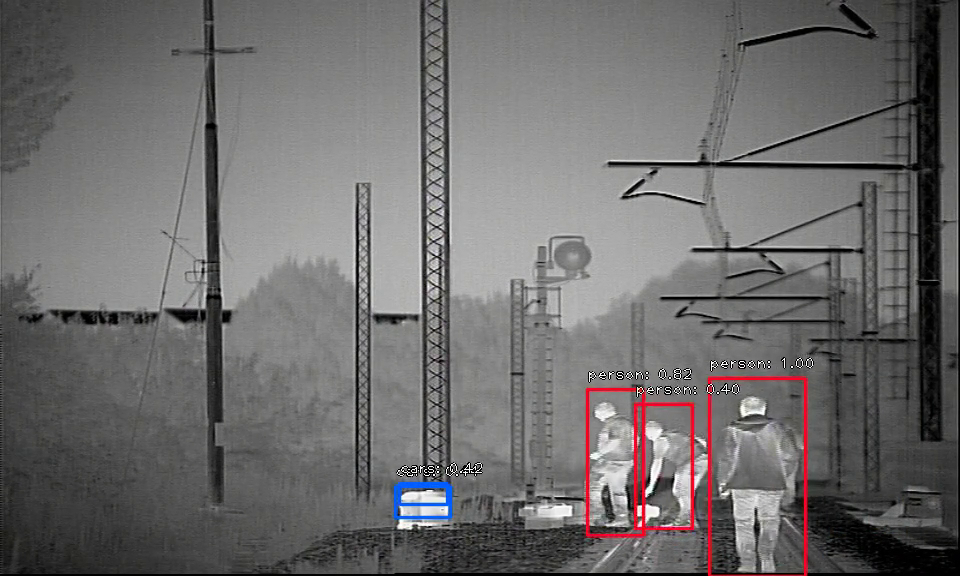
\includegraphics[width =0.99\textwidth]{images/examples/rfi_1_030_1.png}
        }
    \end{minipage}%
    \begin{minipage}{.5\linewidth}
        \centering
        \subfloat[]{
            \label{rfi_030:b}
            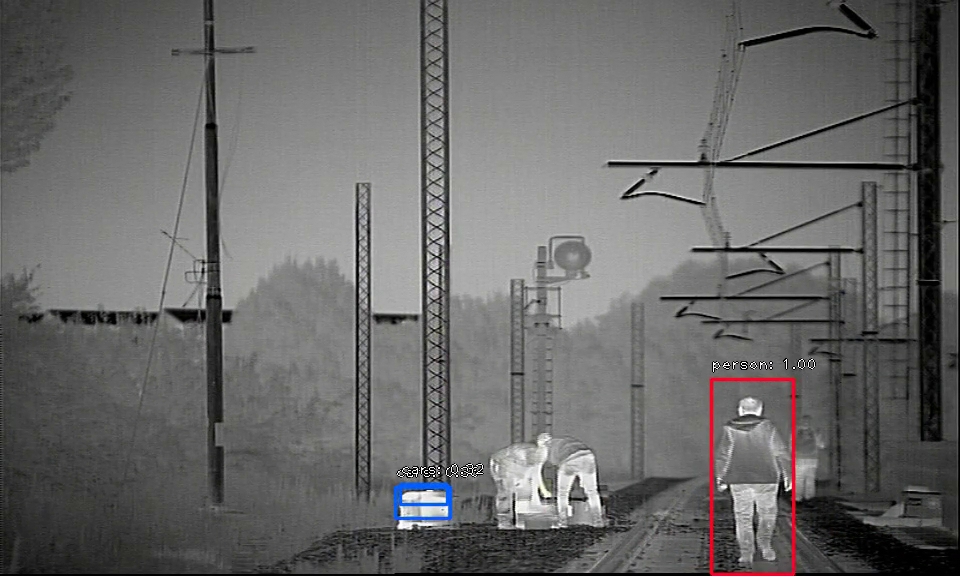
\includegraphics[width = 0.99\textwidth]{images/examples/rfi_1_030_2.png}
            }
    \end{minipage}
    \centering
    \caption{Rilevazioni su video RFI con soglia 0.30}
    \label{fig:rfi_030}
\end{figure}

Questo problema è facilmente risolvibile aumentando la soglia di rilevamento, infatti portandola a $0.8$ si rimuovono la maggior parte dei falsi positivi (Frame in Figura \ref{fig:rfi_080}). 

\begin{figure}[]
    \begin{minipage}{.5\linewidth}
        \centering
        \subfloat[]{
            \label{rfi_080:a}
            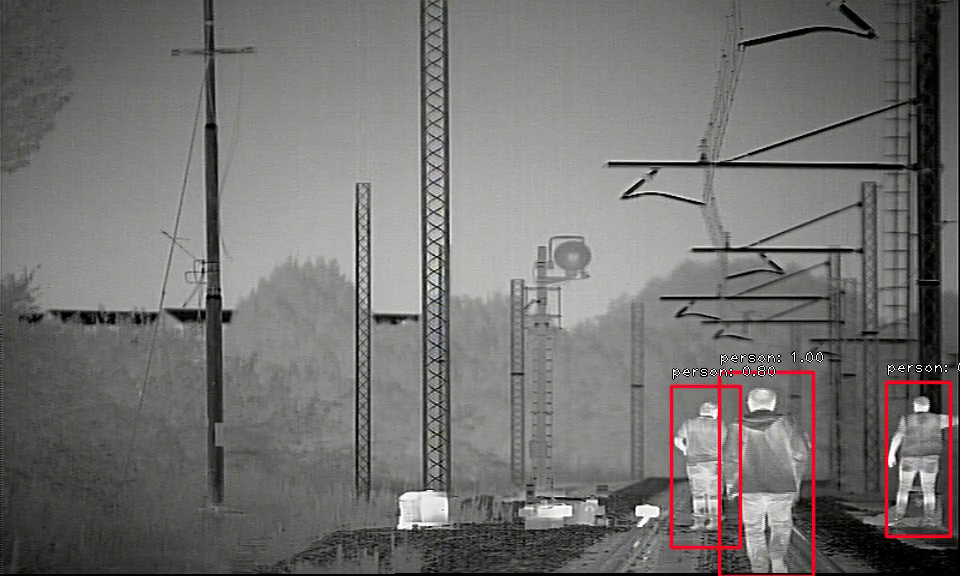
\includegraphics[width =0.99\textwidth]{images/examples/rfi_1_080_1.png}
        }
    \end{minipage}%
    \begin{minipage}{.5\linewidth}
        \centering
        \subfloat[]{
            \label{rfi_080:b}
            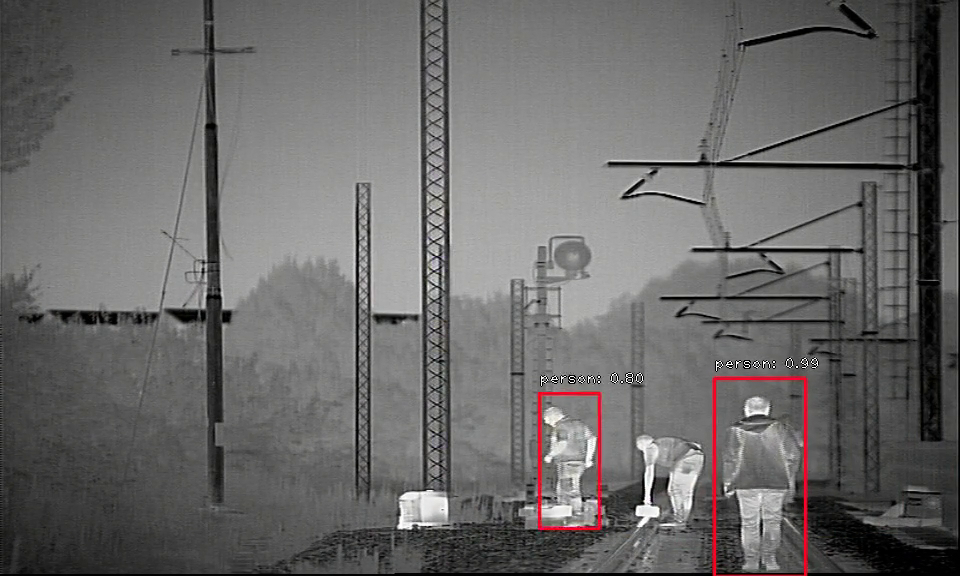
\includegraphics[width = 0.99\textwidth]{images/examples/rfi_1_080_2.png}
            }
    \end{minipage}
    \centering
    \caption{Rilevazioni su video RFI con soglia 0.80}
    \label{fig:rfi_080}
\end{figure}

Un altro problema che rimane però è la rilevazione dei lavoratori in posizioni non usuali, ad esempio quando sono chinati. In Figura \ref{rfi_080:b} vi è un'esempio in quanto l'operaio sembra stia raccogliendo qualcosa per terra e non è stato rilevato. Per risolverlo sono stati annotati alcuni frame di quel video per poi effettuare test su altri due video a nostra disposizione. 
\section{IoU sul tempo}
\label{sec:iou_over_time}
Allo scopo di migliorare precision e recall è stato sviluppato un algoritmo per eliminare rilevazioni fasulle e validare quelle effettivamente presenti. L'algoritmo in questione è in Algoritmo \ref{alg:iou}, mentre l'implementazione in Python è reperibile in Appendice \ref{appendix:a}.


\begin{algorithm}[H]
    \SetAlgoLined
    \SetKwInOut{Input}{Input}\SetKwInOut{Output}{Output}
    \Input{Detection di $N$ immagini, Threshold}
    \Output{Detection di $N$ immagini}
    \KwData{detections, T}
    \KwResult{detections'}
    $ max\_detections \leftarrow max\_detections\_in\_image(detections)$ \;
    $ R\_tree \leftarrow new\_r\_tree() $\;
    \For{$ d \in (detections - max\_detections)$}{
        $R\_tree.insert(d)$\;
    }
    $iou\_values \leftarrow empty\_array(len(max\_detections))$\;
    \For{$ d_i \in max\_detections$}{
        $intersected\_dets \leftarrow R\_tree.find\_intersection(d_i)$\;
        \For{$d_j \in intersected\_dets$} {
            $iou\_values[d_i] \text{ += } compute\_iou(d_i, d_j) $\;
        }
        $iou\_values[d_i] \text{ /= } len(intersected\_dets)$\; 
    }
    $detections' \leftarrow empty\_array(len(detections))$\;
    \For{$d_i \in max\_detections$}{
        \If{$iou\_values[d_i]>T$}{
            $detections'.insert(d_i)$\;
        }
    }
    \Return{$detections'$}
    \caption{Algoritmo di IoU calcolata su diversi frame}
    \label{alg:iou}
\end{algorithm}

L'input dell'algoritmo sono le rilevazioni effettuate su $N$ immagini ed una soglia $T$. 
Il primo passo effettuato è la ricerca dell'immagine contenente più rilevazioni in quanto è quella intuitivamente più soggetta ad avere qualche \ac{BB} trovata erroneamente durante la fase di inferenza. Una volta trovata si inseriscono le detection di tutte le altre immagini all'interno di una struttura che ci permetta di effettuare ricerche su coordinate spaziali in maniera efficiente, ovvero un albero R.
Dopodiché, per ogni immagine che contiene più \ac{BB}, si calcola un valore di \ac{IoU} rispetto a tutte le \ac{BB} delle altre immagini che si intersecano con essa. La \ac{IoU} è un valore compreso tra $0$ e $1$, quindi si normalizza usando il numero di \ac{BB} che intersecano.
Dopo questa fase avremo quindi un array di lunghezza pari al massimo numero di rilevazioni su un'immagine che contiene valori di \ac{IoU}.
Nell'ultima parte dell'algoritmo si confronta ogni valore di questo array per vedere se è superiore alla soglia $T$ passata in input: se lo è la \ac{BB} corrispondente verrà inserita come detection \textit{valida} per ogni immagine nel batch, altrimenti viene scartata.

